To obtain a drop of sweetened water, rats had to wait for a fixed \gls{gt} of 7~s from trial onset before entering the reward area located at the front of the treadmill, while the belt was slowly moving backward (\Autoref{fig:lesion:task}{A}).
Across training sessions composed of $\sim$120~trials, animals learned to wait longer and longer to enter the reward are just after the \gls{gt} and achieve higher percentage of correct trials (\Autoref{fig:lesion:task}{B}, and \autoref{fig:appendix:CorrectTrialCurve}).
Task proficiency was clearly associated with the acquisition and reliable performance of the following routine (\Autoref{fig:lesion:task}{C}):
\begin{enumerate}[noitemsep]
    \item during the intertrial, following the consumption of the reward, rats remained in the reward area;
    \item when the treadmill was turned on (trial onset), they did not move and let the belt carry them away from the reward area;
    \item when they reached the rear wall of the treadmill, they started outrunning the treadmill to reenter the reward area, i.e., the \gls{et} just after 7~s ($ET\geq GT$).
\end{enumerate}
After 2--3 weeks of daily practice, rats used this wait-and-run routine in about 75\% of the trials (\Autoref{fig:lesion:task}{C}, see \autoref{ch:methods:dataAnalysis} for the operational definition of this routine).
Finally, learning this routine was paralleled by a robust invigoration of the running phase of the motor routine toward the reward area (\Autoref{fig:lesion:task}{D}).

\begin{figure}[bth!]
 \begin{center}
	\makebox[\textwidth][c]{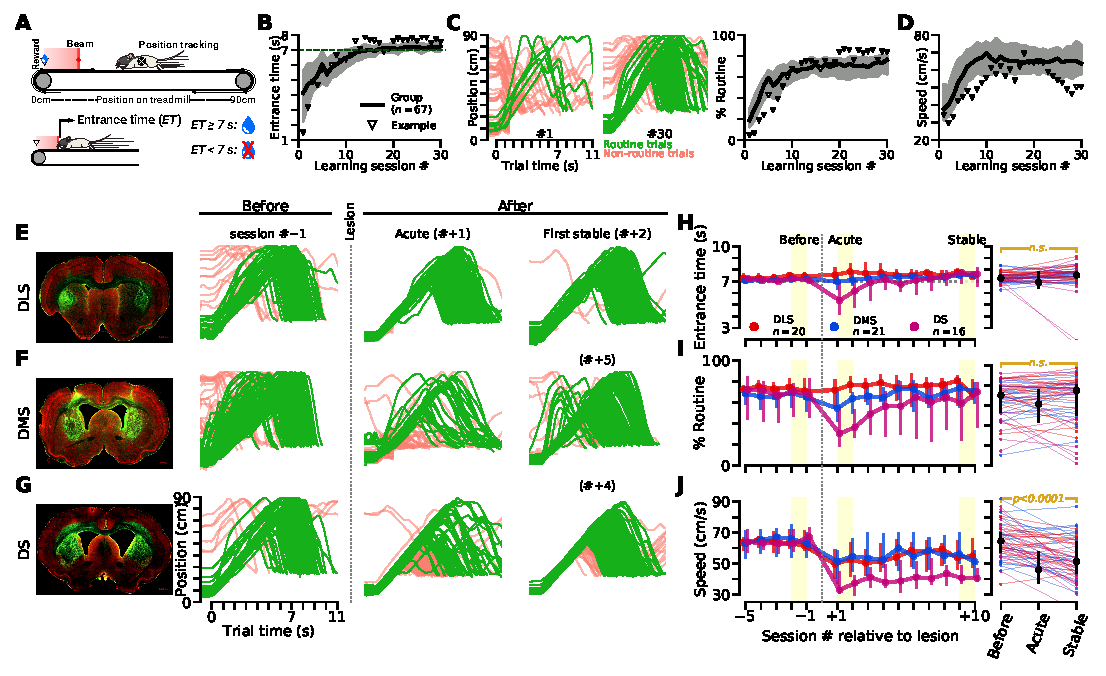
\includegraphics[scale=1]{ch-lesion/figures/Task_Example_Group.pdf}}
	\caption[The Striatum Energizes Motor Routines]
	{\textbf{The striatum is necessary to energize the running component of a motor routine.}
	\textbf{(A)} Experimental apparatus and task rules.
	\textbf{(B-D)} Performance across training sessions and animals.
	Shaded areas represent the 2nd and 3rd quartiles. Triangles represent the changes in performance of an example animal. 
	All the trajectories of this animal during sessions \#1 and \#30 are shown in C (left). 
	\textbf{(E-G)} Histology (1st column, GFAP in green shows gliosis, red is Neun) and trajectories from single animals with bilateral lesions of the dorsolateral, dorsomedial and dorsal striatum (E: DLS, F: DMS: G: DS).
	\# indicates session number relative to lesion break.
	\textbf{(H-J)} Left, Session-by-session time course of the lesion effect on ET (H), percentage of routine usage (I) and speed when animals run toward the reward area (I).
	Right, group data statistical comparison before vs after lesion (10,000 permutations).
	}
	\label{fig:lesion:task}
 \end{center}
\end{figure}
\par
Once the performance was stable, after at least 30 training sessions, we performed fiber-sparing lesions of the striatum ($n=57$ animals, for the lesion protocol, see \autoref{ch:method:lesion}).
The lesions targeted either the \gls{dls} or the \gls{dms}, or both territories, the entire \gls{ds} (\Autoref{fig:lesion:task}{E-G}, see also \autoref{fig:method:LesionSizeLocation}).
Behavioral testing resumed two weeks after the lesion surgery.
Visually, the animals had normal behavior (locomotion, food/water intake) in their homecage at the end of the recovery period.
\par
After the lesion, the behavior of the animals could be divided into an `acute' phase in the first few sessions post-lesion, and a `stable' phase that begins $\sim$9 sessions after the lesion and persists.
This dichotomy does not apply to every animal, apparently animals with bigger lesions have a stronger acute effect.
This can be seen in example animals of \Autoref{fig:lesion:task}{F,~G}, and at the population level in \Autoref{fig:lesion:task}{H}, however, the case illustrated in \Autoref{fig:lesion:task}{E} is an example of a rat with smaller lesion and no acute condition.
To better visualize the acute effect, I grouped the first two post-lesion sessions and presented their average statistics throughout this manuscript.
Similarly, sessions $+9$ and $+10$ were also grouped to represent the stable effect of the lesion.
Animals with this acute effect ran toward the reward area prematurely after trial onset and, consequently, a drop in the usage of the wait-and-run routine was observed during these first post-lesion sessions (\Autoref{fig:lesion:task}{I}).
Surprisingly, most of these animals recovered from this initial impairment and after a few additional sessions, task proficiency was similar to the pre-lesion level (\Autoref{fig:lesion:task}{H-I}, right panels, compare the stable condition to the `before' condition).
Moreover, for most of the animals with a lesion restricted to the DLS and DMS, task proficiency was virtually unaltered when resuming behavioral testing.
We then looked at animals' speed, the velocity with which they outran the opposing treadmill in the third step of the wait-and-run motor routine (see \autoref{ch:methods:dataAnalysis} for the definition).
Strikingly, the animals' speed was irreversibly reduced following striatal lesion (\Autoref{fig:lesion:task}{I}).
In addition, the difference in speed due to lesion was strongly correlated with the size of the lesion (\Autoref{fig:appendix:spd}{A}).
\begin{figure}[tb!]
    \begin{center}
        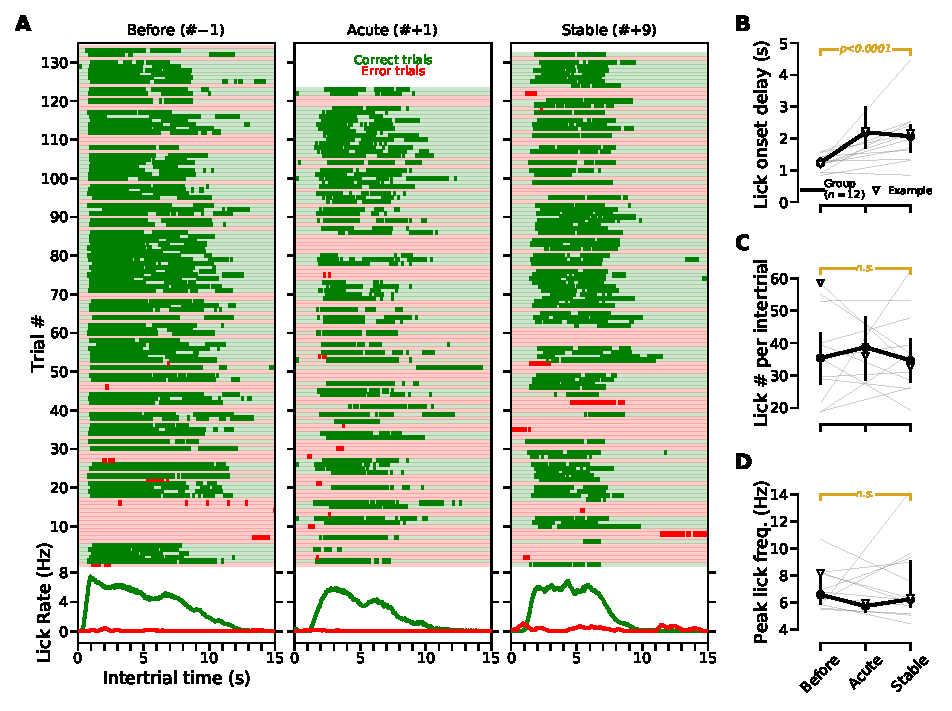
\includegraphics[width=\textwidth]{ch-lesion/figures/Lick.pdf}
        \caption[Licking Behavior After Striatal Lesion]
        {\textbf{Licking behavior mostly unaffected by the striatal lesion.}
        \textbf{A)}
        Trial-by-trial licking pattern (\textit{top}) and averaged lick rate aligned to intertrial onset for a single animal in 3~sessions (1~just before and 2~after lesion).
        Each tick shows one lick in the reward delivery port.
        \textbf{B-D)}
        Effect of striatal lesion on lick onset delay (\textit{B}), number of licks per intertrial (\textit{C}) and peak licking frequency (\textit{D}).
        Same color code for individual lesion type as in \autoref{fig:lesion:task}.
        }
        \label{fig:lesion:lick}
    \end{center}
\end{figure}
Moreover, the maintained task proficiency following striatal lesion suggested that the motivation of the animals to perform the task and to obtain rewards was preserved.
In agreement with this statement, animals with a striatal lesion kept licking the reward after committing correct trials(\Autoref{fig:lesion:lick}{A}).
They licked the number of times after reward delivery and also their peak lick frequency was not affected (\Autoref{fig:lesion:lick}{C-D}).
However, they systematically started to lick later (\Autoref{fig:lesion:lick}{B}).
Much like the speed, this effect was also irreversible, and might be a measure of slower speed in approaching the reward port after crossing the infrared beam (which is $\sim$10~cm from the reward port), or slower postural adjustments to consume the delivered reward.
\par
\begin{figure}[bth!]
 \begin{center}
	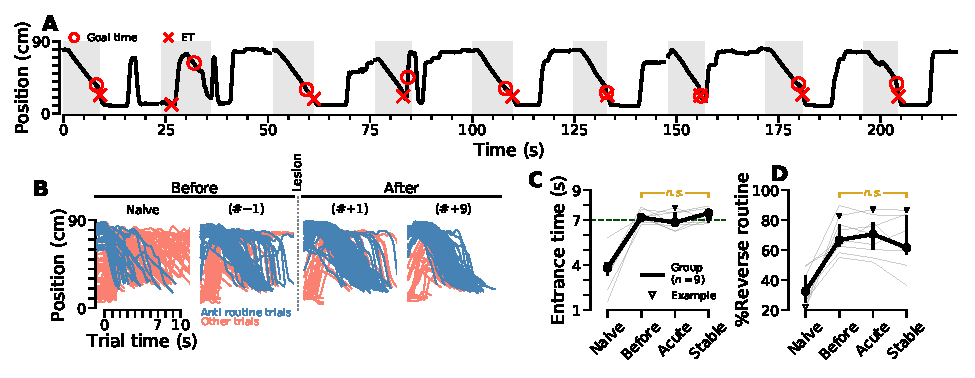
\includegraphics[width=\textwidth]{ch-lesion/figures/ReverseTreadmill.pdf}
	\caption[Preserved Motor Routine Performance After Lesion]
	{\textbf{Preserved performance of the run-and-wait routine following striatal lesion.}
	\textbf{(A)} Trajectory of a proficient animal trained in a version of the timing task in which the belt moved toward the reward area (rather than away from it). 9 consecutive trials and intertrials are shown.
	\textbf{(B)} Trajectories from a single representative animal in two sessions before and two sessions after lesion.
	\textbf{(C-D)} Comparison of ET (C) and percentage of run-and-wait routine usage (D), before and after striatal lesion.
	}
	\label{fig:lesion:rev}
 \end{center}
\end{figure}
These results suggest that the dS is selectively critical for the invigoration of the reward-oriented active component of the wait-and-run routine.
But at this stage, we can not rule out that the transient impairment in performance induced by large dS lesions reflects a deterioration of procedural learning and a reversal to the behavior expressed before routine acquisition (Fig. 1B and C, \cite{Dhawale2019}), compensated in subsequent post-lesion sessions through a dS-independent learning process.
We thus trained a new group of animals in a modified version of the task in which the treadmill belt moved slowly toward the reward area (instead of away from it).
Several animals learned to perform proficiently this version of the task by adopting a run-and-wait routine: they moved to the back of the treadmill during intertrial (after licking the sweetened water from the previous trial and while the belt was immobile) and, following trial onset, they remained immobile while being passively transported toward the reward area (Fig. 2, A to C).
Consequently, after extensive training, animals were positioned away from the reward area at trial onset in a bigger fraction of the trials (Fig. 2, A and D). 
If the dS lesion abolished this procedural learning, we expected animals to start the trials close to the reward area in the first post-lesion session. 
This is not what was observed and, more generally, performance of the run-and-wait routine was spared by dS lesion , Fig. 2, B to D).
A lack of effect of the dS lesion could be due to the fact that learning the run-and-wait routine was easier than learning the wait-and-run routine. 
This is unlikely to be the case as learning to conform to the GT constraint using the run-and-wait routine took a similar number of sessions compared to the wait-and-run routine (fig. S6).







Regarding the aforementioned issue of performance confound, a key feature of this routine is that its first half requires the animals to follow a specific procedure (staying in the reward area after licking the reward, remaining still after treadmill onset until reaching the rear wall) without producing movements. 
Thus, a deficit in performing this routine can only be attributed to altered processes upstream of motor implementation.
In addition, because we used a motorized treadmill, animals were forced to run, at least once they reached the rear wall.
Thus, for the rats, both disengaging from the task (not approaching the reward area during the entire duration of a trial) and incorrect response ($ET<GT$) were associated with expending a significant amount of energy to run (for nothing), a condition that rarely occurred in tasks previously used to probe striatal contribution to the control of purposive actions.
\par


\par
Altogether, these results indicate that the dS is not required to initiate or execute the sequential steps of a learned motor routine but is critical to invigorate its reward-oriented running phase.
To better understand the origin of this vigor deficit, we examined whether the striatal lesions affected the animals' elementary ability to modulate their running speed.
It has been previously shown that the speed of reward-oriented movements increases with movement distance to minimize temporal discounting of rewards \cite{Shadmehr2010JN, Reppert2018JNPhys}.
We compared running speed in trials during which running epochs were initiated from the back versus the middle of the treadmill (Fig. 3A, i.e., long vs short run distance).
As predicted, animals ran faster when they initiated their runs from the back of the treadmill than from its middle (Fig. 3B). This modulation was maintained after dS lesion (Fig. 3B), although running speeds were generally slower following dS lesion.
Next, we compared basic locomotor activity between control and lesioned rats, in a paradigm that did not include reward-oriented runs, using a different treadmill.
The locomotion test consisted of several trials (30~s long) at fixed speeds (0~cm/s to 40~cm/s), interleaved with short breaks (30~s long).
We found that both control and lesioned rats displayed similar exploratory locomotor activity when the treadmill remained immobile (Fig. 3C).
In addition, in trials in which the treadmill was turned on, both groups were similarly able to follow a reasonable range of imposed speeds even though, as the speed increased, animals with a dS lesion ran with slightly slower speeds than control animals (Fig. 3D).
Altogether, this set of experiments indicated that the dS lesion spared the ability of rats to modulate their running speed.
\par
If the dS lesion spared the rats' ability to modulate their running speed, the most parsimonious explanation of our results is that lesioned animals "preferred" slower speeds.
A similar conclusion had been reached when studying the origin of bradykinesia in PD, which led to the proposal that such reluctance to perform fast movements was caused by an increased sensitivity to movement cost (or effort) \cite{Mazzoni2007JN, Baraduc2013JN}.
Could a similar interpretation apply to our results?
To address this question, we took advantage of the optimal control framework that relies on the assumption that animal behavior is optimal with respect to a cost function.
We implemented a simple model to simulate the optimal trajectory of a rat taking into account costs related to locomotion control (effort) and those imposed by the task rules (running in the front is costly as this leads to premature ET, which is penalized).
Two approximations of effort- and task rules-related costs were combined in 4 versions of the models and we found that increasing effort sensitivity consistently resulted in optimal trajectories that were closer to the reward area, hence the combination of late initiation of the run phase with fast speeds not used (Fig. 4A).
This result is not only in agreement with the reduced running speed observed following lesion but is also reminiscent of the behavior observed during the very first post-lesion sessions, when animals with large dS lesion ran mainly close to the reward area (Fig 1, F and G). 
We thus reanalyzed the effect of dS lesion on the trajectory, focusing on animals with a significant reduction in running speed (Fig. 4B, i.e., animals with larger lesion) and on trials during which animals perfectly executed the wait-and-run routine.
Following dS lesion, rats started running forward earlier relative the length of the treadmill (Fig. 4C).
This effect, while being maximal on the first post-lesion sessions, remained significant after three weeks of daily testing (Fig. 4D) and was correlated with lesion size (Fig. 4E).





\begin{figure}[bth!]
 \begin{center}
	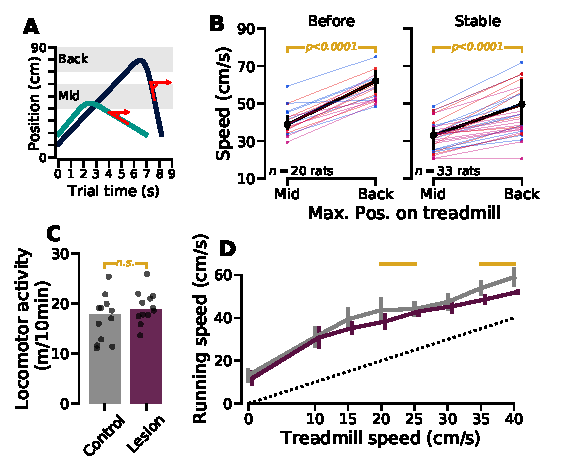
\includegraphics[scale=1]{ch-lesion/figures/MotorPreserved.pdf}
	\caption[Preserved Motor Control After Striatal Lesion]
	{\textbf{Preserved modulation of running speed and spontaneous locomotor activity following striatal lesion.}
	\textbf{(A)} Average speed when rats ran toward the reward area. Data were split according to the position of the rats on the treadmill when initiating their runs.
	\textbf{(B)} Speed of runs initiated either in the back or the middle portion of the treadmill calculated for each animal on the last 5 sessions before lesion (left) and sessions \#4 to \#9 after lesion (right).
	\textbf{(C)} Distance ran while exploring a new immobile treadmill for non-lesioned and lesioned rats ($n=12$).
	\textbf{(D)} Average running speed in a free running task (no reward) in which control and lesioned rats were submitted to trials with incremental treadmill speed (same color code as in C).
	Horizontal golden lines indicated significant differences between groups.
	}
	\label{fig:lesion:motorOk}
 \end{center}
\end{figure}

\begin{figure}[bth!]
	\begin{center}
		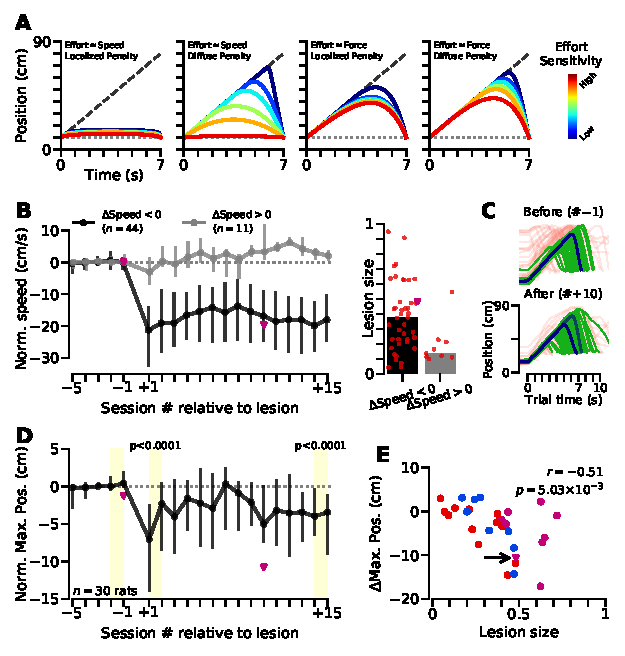
\includegraphics[scale=1]{ch-lesion/figures/MaxPosAnalysis.pdf}
		\caption[Optimal Trajectory and Experimental Validation]
		{\textbf{Optimal trajectory vs.\ effort sensitivity and experimental validation.}
		\textbf{A)}
		Optimal trajectories predicted by models with different effort and spatial costs approximations.
		The cost of premature entrance in the reward area (spatial cost) was simulated using a Heaviside function that was either localized ($\sim$step function with non-zero value within the reward area) or diffuse ($\sim$a sigmoid function whose value gradually decreases toward zero away from the reward area).
		Effort was approximated as the square value of either the modeled muscular force produced by the animals or of its speed.
		\textbf{B)}
		\textit{Left}: animals were divided into two groups based on the impact of the striatal lesion on their running speed.
		\textit{Right}: lesion size for animals in those two groups.
		Green triangles in panels~B,~D, and~E are data points from the example animal whose trajectories, before and after lesion, are shown in panel~C.
		\textbf{C)}
		Effect of striatal lesion on the trajectories of a single animal.
		Only trials in which the routine was executed (thin blue lines) were taken into account to find the trajectory of median maximum position (tick blue line).
		The shadow of the trajectory of median maximum position before lesion is displayed in the bottom plot for comparison.
		\textbf{D)}
		Effect of striatal lesion on the median maximum position in routine trials.
		\textbf{E)}
		Effect of striatal lesion on the median maximum position vs.\ lesion size.
		Same color code for individual lesion type as in \autoref{fig:lesion:task}.
		}
		\label{fig:lesion:maxPos}
	\end{center}
\end{figure}

\begin{figure}[bth!]
	\begin{center}
		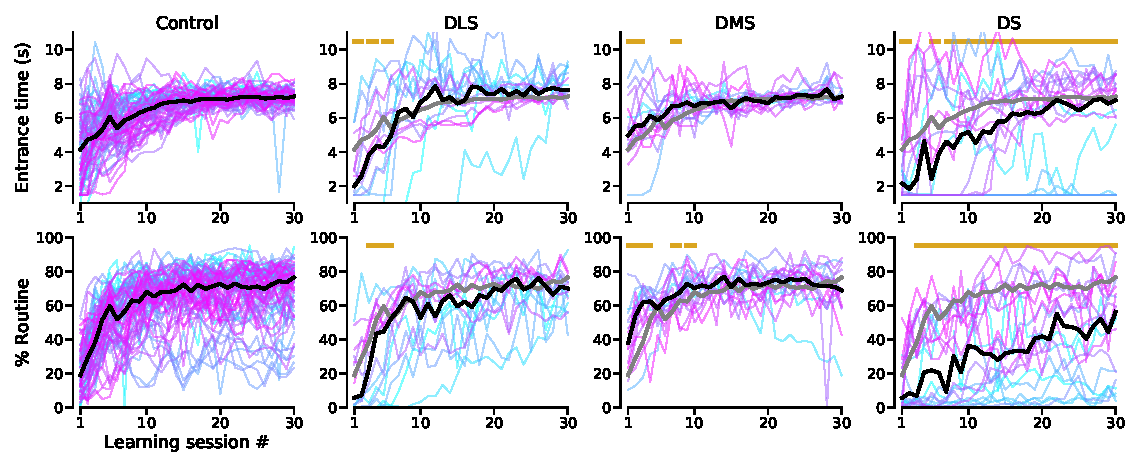
\includegraphics[width=\textwidth]{ch-lesion/figures/EarlyLesionLearning.pdf}
		\caption[Effects of Striatal Lesions on Learning]
		{\textbf{Effect of DLS, DMS and DS lesions performed before training on task learning.}
		\textbf{A)} Session-by-session change in performance ($ET$, upper panels; Percentage of trials in which the routine was used, lower panels) for animals without lesion (Control, \textit{left}) and for animals that received a lesion before training (DLS, DMS, DS from left to \textit{right}).
		Black lines indicate Control group median.
		Thin colored lines indicate single animals.
		Thick colored lines (same color code as in \autoref{fig:lesion:task}) in 3 rightmost columns indicate group performance for comparison (8 lesion animals with fewer than 30 training sessions are not shown, which explains the difference in the number of animals in this figure and \autoref{fig:method:LesionSizeLocation}).
		Horizontal golden lines indicate significant differences between control and lesion groups (corrected for multiple comparisons).
		\textbf{B)} Trajectories before and after extensive training (sessions \#1 and \#30) for two animals with large DS lesions.
		Note that, after extensive practice, R238 was capable of performing the wait-and-run routine.
		\textbf{C)} Percentage of trials in which animals remained in the front region of the treadmill (computed for sessions \#25 to \#30) versus lesion size.
		}
		\label{fig:lesion:EarlyLesionLearning}
	\end{center}
\end{figure}